\question{5.2}{Een vulmachine vult pakken rijst waarop staat dat daarin $1 000$ gram rijst zit.
Omdat er altijd wat variatie zit in de afgeleverde hoeveelheden, staat de machine ingesteld op een gemiddeld vulgewicht van $1 010$ gram.
We mogen ervan uitgaan dat de afgeleverde hoeveelheden beschreven worden door een normale verdeling met $\mu = 1 010$ gram.
De standaarddeviatie is echter onbekend.}

\begin{enumerate}[label=(\alph*)]
    \item Bij nauwkeurig nawegen van een groot aantal pakken bleek dat in $20\%$ van de gevallen een pak minder dan $1 000$ gram rijst bevat.
    Bereken op basis van deze informatie de standaarddeviatie van de vulgewichten.
    \answer{
        Laat $X$ de normaal verdeelde kansvariabele zijn met verwachtingswaarde $\mu=1 010$ en onbekende standaarddeviatie $\sigma$ die het gewicht van een pak rijst beschrijft.
        In dat geval is de kansvariabele $Z = \frac{X - \mu}{\sigma}$ standaardnormaal verdeeld, oftewel $Z \sim N(0, 1)$.
        
        De $z$-waarde waarvoor geldt dat $P(Z < z) = 0,20$ is gelijk aan
        \[
            z = \text{InvNorm}(opp=0,20; \mu=0; \sigma=1) \approx -0,8416.
        \]
        
        In andere woorden: de waarde $1 000$ g ligt 0,8416 standaarddeviaties onder het gemiddelde, oftewel:
        \[
            \frac{1 000 - 1 010}{\sigma} = -0,8416 \rightarrow 1 000 = 1 010 - 0,8416 \cdot \sigma \rightarrow \sigma \approx 11,8818
        \]

        \begin{center}
            \resizebox{0.9\textwidth}{!}{
                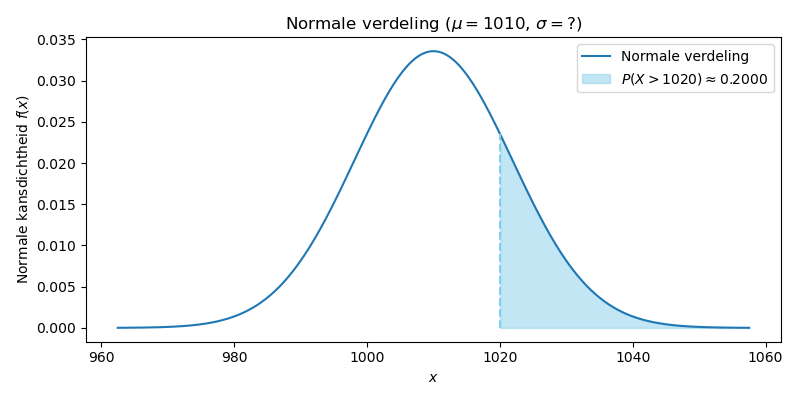
\includegraphics{opg5.2a.png}
            }
        \end{center}
    }

    \item Hoe groot is de kans dat een willekeurig pak rijst meer weegt dan $1 020$ gram?
    \answer{
        Zodra we de verwachtingswaarde $\mu$ en de standaarddeviatie $\sigma$ van een normale verdeling weten, is het niet meer moeilijk om een kans te bepalen:
        De kans dat een willekeurig pak rijst meer dan $1 020$ gram weegt is gelijk aan:
        \begin{align*}
            P(X > 1 020)    &= \text{normalcdf}(a=1 020; b=10^{10}; \mu=1 010; \sigma=11,8818) \\
                            &\approx 0,20.
        \end{align*}
        Merk op dat deze kans hetzelfde is als de kans $P(X < 1 000)$, aangezien de kansverdeling van $X$ symmetrisch is rond $\mu = 1 010$.
        \begin{center}
            \resizebox{0.9\textwidth}{!}{
                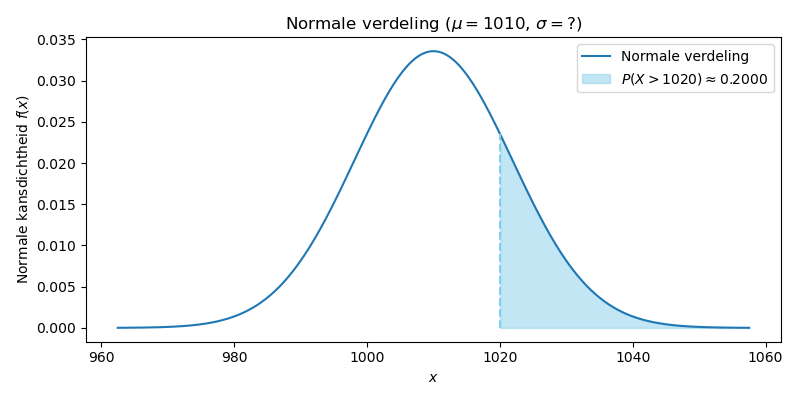
\includegraphics{opg5.2b.png}
            }
        \end{center}
    }

    \item Stel we kiezen willekeurig $16$ pakken rijst.
    Hoe groot is de kans dat deze gemiddeld minder dan $1 000$ gram rijst bevatten?
    \answer{
        Laat $X_1, X_2, \ldots, X_16$ de gewichten zijn van $16$ willekeurig gekozen pakken rijst.
        Volgens de centrale limietstelling geldt dat het gemiddelde $\overline{X} = \frac{X_1+X_2+\ldots+X_{16}}{16}$ van deze gewichten opnieuw normaal verdeeld is met verwachtingswaarde $\mu=1 010$ en standaardafwijking $\frac{\sigma}{\sqrt{16}} = \frac{\sigma}{4} \approx 2,9705$.
        De kans dat de $16$ willekeurig gekozen pakken rijst gemiddeld minder dan $1 000$ gram rijst bevatten is gelijk aan:
        \begin{align*}
            P(\overline{X} < 1 000)     &= \text{normalcdf}(a=-10^{10};b=1 000;\mu=1 010;\sigma=2,9705) \\
                                        &\approx 3,8072 \cdot 10^{-4}.
        \end{align*}
    }
\end{enumerate}
